\documentclass{beamer}
%\definecolor{envy}{HTML}{1A936F}
%\definecolor{berry}{HTML}{C6878F}
%\definecolor{turq}{HTML}{077187}
%\definecolor{pgreen}{HTML}{CBE896}
%\definecolor{db}{HTML}{074F57}
%\colorlet{ldb}{db!55!white}
%\colorlet{lpgreen}{pgreen!55!white}

\definecolor{envy}{HTML}{1A936F}
%\definecolor{berry}{HTML}{E3463F}
\definecolor{berry}{HTML}{DDE6CB}
\definecolor{turq}{HTML}{077187}
\definecolor{pgreen}{HTML}{FD9564}
\definecolor{db}{HTML}{213862}
\colorlet{ldb}{db!55!white}
\colorlet{lpgreen}{pgreen!55!white}
\newcommand{\light}[1]{\textcolor{db!50!white}{#1}}
% New colours!
% \setbeamercolor{background canvas}{bg=GreyWhite}

\setbeamercolor{title}{fg=db, bg=pgreen!55!white}
\setbeamercolor{frametitle}{fg=db, bg=pgreen!55!white}
\setbeamercolor{normal text}{fg=db}
\setbeamercolor{block title}{fg=db,bg=pgreen!55!white}
%%\setbeamercolor{title}{fg=black, bg=pgreen!55!white}
%%\setbeamercolor{frametitle}{fg=black, bg=pgreen!55!white}
%%\setbeamercolor{normal text}{fg=black}
%%\setbeamercolor{block title}{fg=black,bg=pgreen!55!white}
%%\setbeamercolor{block body}{fg=black!22!white}
%\setbeamercolor{alerted text}{fg=Pinky}
\setbeamercolor{itemize item}{fg=turq}
\setbeamercolor{itemize subitem}{fg=db!85!white}
\setbeamercolor{itemize subsubitem}{fg=db!85!white}
%\setbeamercolor{framesource}{fg=Carrot}
%\setbeamercolor{section in toc}{fg=PurpNav}
\setbeamercolor{footnote}{fg=black}
\setbeamercolor{footnote mark}{fg=black}
\setbeamercolor{myfootlinetext}{fg=black}
\setbeamertemplate{itemize subitem}{fg=turq}
\setbeamertemplate{itemize subsubitem}{fg=turq}
%\setbeamertemplate{itemize item}{\color{DarkPurple}$\blacksquare$}
%\setbeamertemplate{itemize item}{\color{DarkPurple}}[circle]
\setbeamertemplate{itemize item}[circle]

\newcommand{\be}{\begin{enumerate}}
	\newcommand{\ee}{\end{enumerate}}
\newcommand{\bi}{\begin{itemize}}
	\newcommand{\ei}{\end{itemize}}
\newcommand{\ccbb}{\cellcolor{turq!15!white}}
\newcommand{\cc}{\cellcolor{pgreen!55!white}}
\newcommand{\ccb}{\cellcolor{berry!35!white}}

% source at bottom left of slide
\newcommand{\sourceleft}[1]{\begin{textblock*}{4cm}(0.3cm,8.8cm)
		\begin{beamercolorbox}[ht=0.5cm,left]{framesource}
			\usebeamerfont{framesource}\usebeamercolor[fg]{framesource}
			{#1}
		\end{beamercolorbox}
	\end{textblock*}}
	
	% source at bottom right of slide
	\newcommand{\sourceright}[1]{\begin{textblock*}{}
			\begin{beamercolorbox}[ht=0.5cm,left]{framesource}
				\usebeamerfont{framesource}\usebeamercolor[berry]{framesource}
				{#1}
			\end{beamercolorbox}
		\end{textblock*}}
		
		\newcommand{\cfcite}[1]{\footnote{\citeauthor{#1}, \citeyear{#1}}}
		
		\newcommand{\sourceextremeright}[1]{\begin{textblock*}{4cm}(10.6cm,8.8cm)
				\begin{beamercolorbox}[ht=0.5cm,left]{framesource}
					\usebeamerfont{framesource}\usebeamercolor[fg]{framesource}
					{#1}
				\end{beamercolorbox}
			\end{textblock*}}
			
			\usetheme{boxes}
			\usepackage[absolute,overlay]{textpos}
			%\usecolortheme{beaver}
			\useinnertheme{circles}
			\usepackage{amsmath}
			\usepackage{amssymb}
			\usepackage{lmodern}
			\usepackage{xcolor}
			\usepackage{tikz-cd}
			\usepackage{tikz}
			\usetikzlibrary{arrows.meta}
			\usetikzlibrary{decorations.markings}
			\usetikzlibrary{calc, arrows}
			\usepackage{longtable}
			\usepackage{graphicx}% http://ctan.org/pkg/graphicx
			\usepackage{booktabs}
			\usepackage{xspace}
			\usepackage{varwidth}
			\usepackage{array} %make columns all same width
			\newcolumntype{C}{>{\centering\arraybackslash}p{0.2\linewidth}}
			\usepackage{scrtime} % for \thistime (this package MUST be listed first!)
			\usepackage{amsmath} % essential for cases environment
			\usepackage{amsthm} % for theorems and proofs
			\usepackage{amsfonts} % mathbb
			\usepackage{graphics,graphicx}
			\usepackage{multirow} % fancy tables
			\usepackage{wasysym} % circle symbols (including half-filled circles)
			\usepackage{enumerate} % fancier enumeration (e.g., a,b,c, ...)
			%\usepackage{xcolor}
			\usepackage{color}
			\usepackage{xstring}
			\usepackage[linguistics]{forest}
			\usetikzlibrary{calc, arrows}
			\usepackage{xcolor,colortbl}
			\usepackage[export]{adjustbox}
			\usepackage{array} %to uncover one col at a time of a table
			%\colorlet{grey}{black!10}
			%below adds slide number without putting total number of slides
			\setbeamertemplate{footline}{%
				\raisebox{8pt}{\makebox[\paperwidth]{\hfill\makebox[10pt]{\scriptsize\insertframenumber}}}}
			
			\newenvironment{itmenv}{\only{\setbeamercolor{local structure}{fg=gray}}}{}
			\setbeamertemplate{enumerate items}[default]
			\setbeamercolor*{enumerate item}{fg=db}
			
			\setbeamercolor*{enumerate subitem}{fg=db}
			
			\newcommand\FrameText[1]{%
				\begin{textblock*}{\paperwidth}(0pt,\textheight)
					\raggedleft #1\hspace{4em}\vspace{20em}
				\end{textblock*}}
				
				\mode<presentation>
				\title{\Huge Spatial Patterns of Molecular Trends in Bacterial Genomes}
				
				\author[Daniella Lato]{\\ \textbf{Daniella Lato}\\ PhD Candidate \\ Golding Lab McMaster University \\ latodf@mcmaster.ca \\ OE3C: Evolutionary Biology/Molecular Evolution \\ May 4, 2019}
				\date[2017]{}
				\IfFileExists{upquote.sty}{\usepackage{upquote}}{}
				\newcommand{\itm}{\item<itm@1->}
				\newcommand{\btVFill}{\vskip0pt plus 1filll}
				\newcommand{\s}{\textit{Sinorhizobium}\ }
				\newcommand{\sm}{\textit{Sinorhizobium meliloti}\xspace}
				\newcommand{\salm}{\textit{Salmonella enterica}\xspace}
				\newcommand{\smel}{\textit{S.\,meliloti}\xspace}
				\newcommand{\smed}{\textit{S.\,medicae}}
				\newcommand{\sfred}{\textit{S.\,fredii}}
				\newcommand{\ssah}{\textit{S.\,saheli}}
				\newcommand{\ster}{\textit{S.\,terangae}}
				\newcommand{\ag}{\textit{Agrobacterium tumefaciens }}
				\newcommand{\p}{progressiveMauve\xspace}
				\newcommand{\agro}{\textit{A.\,tumefaciens }}
				\newcommand{\bur}{\textit{Burkholderia}\xspace}
				\newcommand{\vib}{\textit{Vibrio}\xspace}
				\newcommand{\bor}{\textit{Bordetella}\xspace}
				\newcommand{\xan}{\textit{Xanthomonas}\xspace}
				\newcommand{\sul}{\textit{Sulfolobus}\xspace}
				\newcommand{\ent}{\textit{Enterobacteria}\xspace}
				\newcommand{\bac}{\textit{Bacillus subtilis}\xspace}
				\newcommand{\ecoli}{\textit{Escherichia coli}\xspace}
				\newcommand{\lis}{\textit{Listeria monocytogenes}\xspace}
				\newcommand{\bass}{\textit{B.\,subtilis}\xspace}
				\newcommand{\bas}{\textit{Bacillus subtilis}\xspace}
				\newcommand{\tub}{\textit{Mycobacterium tuberculosis}\xspace}
				\newcommand{\strep}{\textit{Streptomyces}\xspace}
				\newcommand{\agrot}{\textit{Agrobacterium tumefaciens}\xspace}
				\newcommand{\ecol}{\textit{E.\,coli}\xspace}
				\newcommand{\salb}{\textit{S.\,alblus}\xspace}
				\newcommand{\salbus}{\textit{S.\,albus}\xspace}
				\newcommand{\shyg}{\textit{S.\,hygroscopicus}\xspace}
				\newcommand{\sliv}{\textit{S.\,lividans}\xspace}
				\newcommand{\sros}{\textit{S.\,roseosporus}\xspace}
				\newcommand{\ssir}{\textit{S.\,sirex}\xspace}
				\newcommand{\sven}{\textit{S.\,venezuelae}\xspace}
				\newcommand{\scoe}{\textit{S.\,coelicolor}\xspace}
				\newcommand{\hal}{\textit{Haloquadratum walsbyi}\xspace}
				\newcommand{\pa}{pSymA\xspace}
				\newcommand{\pb}{pSymB\xspace}
				\setbeamertemplate{navigation symbols}{}
				\newcommand*{\NodeSize}{0.5cm}%
				\newcommand*{\YShiftBetweenRows}{-1cm}% Subsequent rows are shited down so they don't overlap
				\tikzset{DNA Style/.style={minimum size=0.5cm, draw=gray, line width=1pt}}{}
				\providecommand{\e}[1]{\ensuremath{\times 10^{#1}}}
				\newlength{\YShift}% 
				\newcounter{ColumnCounter}% Prefix for node labels
				
				\newcommand\FourQuad[4]{%
					\begin{minipage}[b][.35\textheight][t]{.47\textwidth}#1\end{minipage}\hfill%
					\begin{minipage}[b][.35\textheight][t]{.47\textwidth}#2\end{minipage}\\[0.5em]
					\begin{minipage}[b][.35\textheight][t]{.47\textwidth}#3\end{minipage}\hfill
					\begin{minipage}[b][.35\textheight][t]{.47\textwidth}#4\end{minipage}%
				}
				
				% Initialize - These are probably not needed, but prefer to set them
				\setlength{\YShift}{0cm}% 
				\setcounter{ColumnCounter}{0}
				
				
				%%%%%%%%%%%%%%%%%%%%%%%%%%%%%%%%%%%%%%%%%%%%%%%%%%%%%%%%%%%%%%%%%%%%%%%%%%%%%%%%%%%%%%%%%%%%%%%%%%%%%%%%%%%%%%%%%%%%%%%%%%%%%%%%%%%%%%%%%%%%%%%%%%%%%%%%%%%%%%%%
				
				
\begin{document}
\begin{frame}
	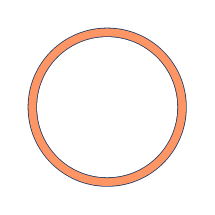
\begin{tikzpicture}[radius=10mm]
	\fill[db] (0,0) circle (10.1mm);
	\foreach \i [count=\ii from 0] in {pgreen, pgreen, pgreen, pgreen}
	\fill[\i] (0,0) -- (\ii*90:10mm)
	arc[start angle=\ii*90,delta angle=90]
	-- cycle;
	\fill[db] (0,0) circle (9mm);
	\fill[white] (0,0) circle (8.9mm);
	%second circle
	%	\foreach \i [count=\ii from 0] in {db, berry, berry}
	%	\fill[\i] (1,0) -- (\ii*120:32mm)
	%	arc[start angle=\ii*120,delta angle=120]
	%	-- cycle;
	%	\fill[white] (1,0) circle (30mm);
	\end{tikzpicture}
	
\end{frame}

\begin{frame}
	
\begin{tikzpicture}[radius=10mm]
	\fill[db] (0,0) circle (10.1mm);
	\foreach \i [count=\ii from 0] in {db, db, db, db}
	\fill[\i] (0,0) -- (\ii*90:10mm)
	arc[start angle=\ii*90,delta angle=90]
	-- cycle;
	\fill[db] (0,0) circle (9mm);
	\fill[white] (0,0) circle (8.9mm);
	%second circle
	%	\foreach \i [count=\ii from 0] in {db, berry, berry}
	%	\fill[\i] (1,0) -- (\ii*120:32mm)
	%	arc[start angle=\ii*120,delta angle=120]
	%	-- cycle;
	%	\fill[white] (1,0) circle (30mm);
	\end{tikzpicture}
	
\end{frame}


\begin{frame}
	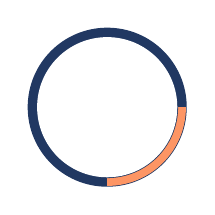
\begin{tikzpicture}[radius=10mm]
	\fill[db] (0,0) circle (10.1mm);
	\foreach \i [count=\ii from 0] in {db, db, db, pgreen}
	\fill[\i] (0,0) -- (\ii*90:10mm)
	arc[start angle=\ii*90,delta angle=90]
	-- cycle;
	\fill[db] (0,0) circle (9mm);
	\fill[white] (0,0) circle (8.9mm);
	%second circle
	%	\foreach \i [count=\ii from 0] in {db, berry, berry}
	%	\fill[\i] (1,0) -- (\ii*120:32mm)
	%	arc[start angle=\ii*120,delta angle=120]
	%	-- cycle;
	%	\fill[white] (1,0) circle (30mm);
	\end{tikzpicture}
	
\end{frame}


\begin{frame}
	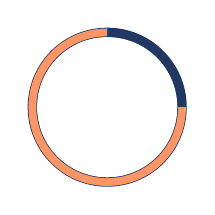
\begin{tikzpicture}[radius=10mm]
	\fill[db] (0,0) circle (10.1mm);
	\foreach \i [count=\ii from 0] in {db, pgreen, pgreen, pgreen}
	\fill[\i] (0,0) -- (\ii*90:10mm)
	arc[start angle=\ii*90,delta angle=90]
	-- cycle;
	\fill[db] (0,0) circle (9mm);
	\fill[white] (0,0) circle (8.9mm);
	%second circle
	%	\foreach \i [count=\ii from 0] in {db, berry, berry}
	%	\fill[\i] (1,0) -- (\ii*120:32mm)
	%	arc[start angle=\ii*120,delta angle=120]
	%	-- cycle;
	%	\fill[white] (1,0) circle (30mm);
	\end{tikzpicture}
	
\end{frame}

	\begin{frame}
		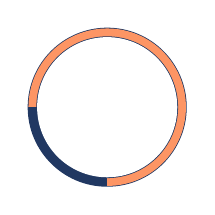
\begin{tikzpicture}[radius=10mm]
		\fill[db] (0,0) circle (10.1mm);
		\foreach \i [count=\ii from 0] in {pgreen, pgreen, db, pgreen}
		\fill[\i] (0,0) -- (\ii*90:10mm)
		arc[start angle=\ii*90,delta angle=90]
		-- cycle;
		\fill[db] (0,0) circle (9mm);
		\fill[white] (0,0) circle (8.9mm);
		%second circle
		%	\foreach \i [count=\ii from 0] in {db, berry, berry}
		%	\fill[\i] (1,0) -- (\ii*120:32mm)
		%	arc[start angle=\ii*120,delta angle=120]
		%	-- cycle;
		%	\fill[white] (1,0) circle (30mm);
		\end{tikzpicture}
		
	\end{frame}


\begin{frame}
	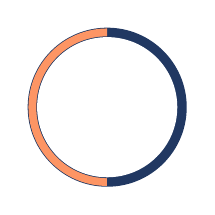
\begin{tikzpicture}[radius=10mm]
	\fill[db] (0,0) circle (10.1mm);
	\foreach \i [count=\ii from 0] in {db, pgreen, pgreen, db}
	\fill[\i] (0,0) -- (\ii*90:10mm)
	arc[start angle=\ii*90,delta angle=90]
	-- cycle;
	\fill[db] (0,0) circle (9mm);
	\fill[white] (0,0) circle (8.9mm);
	%second circle
	%	\foreach \i [count=\ii from 0] in {db, berry, berry}
	%	\fill[\i] (1,0) -- (\ii*120:32mm)
	%	arc[start angle=\ii*120,delta angle=120]
	%	-- cycle;
	%	\fill[white] (1,0) circle (30mm);
	\end{tikzpicture}
	
\end{frame}


\begin{frame}
	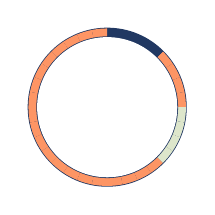
\begin{tikzpicture}[radius=10mm]
	\fill[db] (0,0) circle (10.1mm);
	\foreach \i [count=\ii from 0] in {pgreen, pgreen, pgreen, pgreen, db, db, db, db, pgreen, pgreen, pgreen, pgreen, pgreen, pgreen, pgreen, pgreen, pgreen, pgreen, pgreen, pgreen, pgreen, pgreen, pgreen, pgreen, pgreen, pgreen, pgreen, pgreen, berry, berry, berry, berry}
	\fill[\i] (0,0) -- (\ii*11.25:10mm)
	arc[start angle=\ii*11.25,delta angle=11.25]
	-- cycle;
	\fill[db] (0,0) circle (9mm);
	\fill[white] (0,0) circle (8.9mm);
	%second circle
	%	\foreach \i [count=\ii from 0] in {db, berry, berry}
	%	\fill[\i] (1,0) -- (\ii*120:32mm)
	%	arc[start angle=\ii*120,delta angle=120]
	%	-- cycle;
	%	\fill[white] (1,0) circle (30mm);
	\end{tikzpicture}
	
\end{frame}

\begin{frame}
	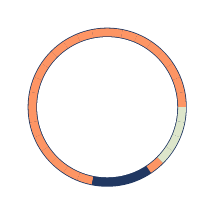
\begin{tikzpicture}[radius=10mm]
	\fill[db] (0,0) circle (10.1mm);
	\foreach \i [count=\ii from 0] in {pgreen, pgreen, pgreen, pgreen, pgreen, pgreen, pgreen, pgreen, pgreen, pgreen, pgreen, pgreen, pgreen, pgreen, pgreen, pgreen, pgreen, pgreen, pgreen, pgreen, pgreen, pgreen, pgreen, db, db, db, db, pgreen, berry, berry, berry, berry}
	\fill[\i] (0,0) -- (\ii*11.25:10mm)
	arc[start angle=\ii*11.25,delta angle=11.25]
	-- cycle;
	\fill[db] (0,0) circle (9mm);
	\fill[white] (0,0) circle (8.9mm);
	%second circle
	%	\foreach \i [count=\ii from 0] in {db, berry, berry}
	%	\fill[\i] (1,0) -- (\ii*120:32mm)
	%	arc[start angle=\ii*120,delta angle=120]
	%	-- cycle;
	%	\fill[white] (1,0) circle (30mm);
	\end{tikzpicture}
	
\end{frame}


\end{document}